\documentclass{article}
\usepackage[utf8]{inputenc}
\usepackage{graphicx}
\graphicspath{ {./images/} }
\usepackage{listings}

\title{CS 590 Assignment 6}
\author{Luke Jiang (jiang700@purdue.edu) }
\date{April 13, 2021}

\begin{document}

\maketitle

\section{Question 1}
According to S3 packet creation page:\\
Versioning is a means of keeping multiple variants of an object in the same bucket. You can use versioning to preserve, retrieve, and restore every version of every object stored in your Amazon S3 bucket. With versioning, you can easily recover from both unintended user actions and application failures.

\section{Question 2}
We can upload files of any type into S3, but the file size muse be smaller than 160GB.

\section{Question 3}
This extra step helps avoid deleting files in accident.

\section{Screenshot}
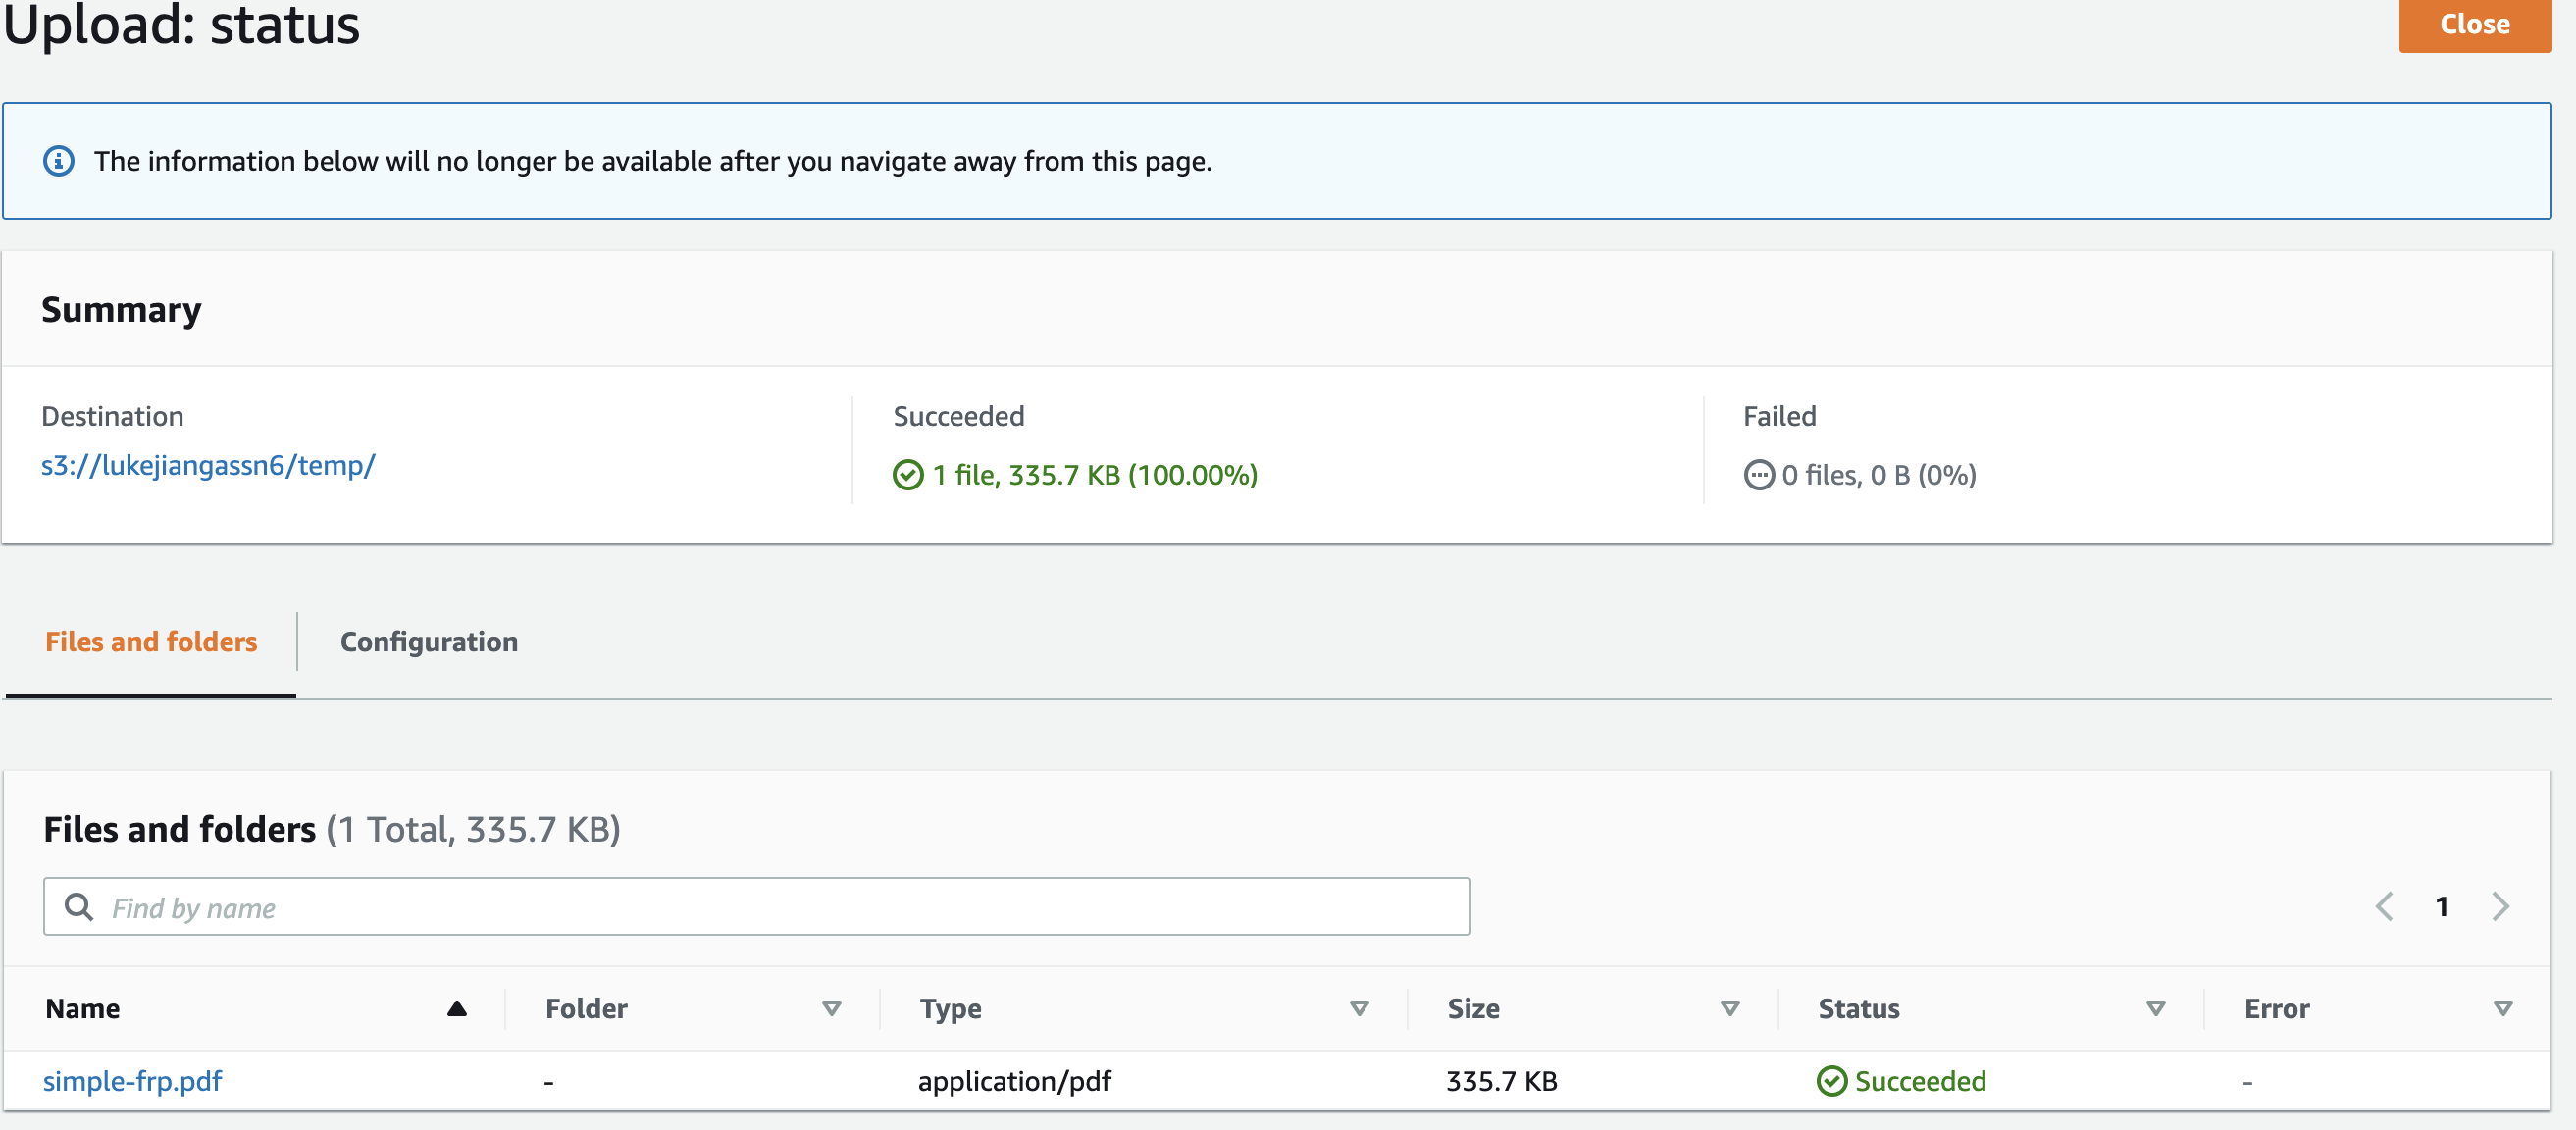
\includegraphics[scale=0.33]{ass6-1.png}

\end{document}